\chapter{Estrategia general del análisis}
% \addcontentsline{toc}{chapter}{Estrategia general del análisis}
\chaptermark{Estrategia general del análisis}



El análisis para el cual está orientada esta tesis, consiste en la búsqueda de Supersimetría en eventos con un fotón aislado muy energético, jets y gran cantidad de energía faltante (cita fran y ultimos articulos). La estrategia general consiste en el conteo del número de eventos observado en exceso sobre el SM, en una cierta región del espacio de observables, rica en eventos de la señal considerada.


\section{Identificación de eventos de fondo}

Para un correcto procedimiento, es necesario conocer los procesos del SM que tengan un estado final equivalente a de la señal buscada. Estos eventos toman el rol de fondo en el contexto de un analisis de búsqueda de SUSY. Para este análisis, son procesos que tienen un fotón, jets y energía faltante en el estado final, y pueden dividirse en varias categorías. Por un lado, los procesos que dan lugar a eventos con un fotón y energía faltante
real, es decir, los que llamamos fondos irreducibles. Estos son:

\begin{itemize}

	\item $Z(\rightarrow \nu\nu)$ + $\gamma$

	\item $W (\rightarrow l\nu)$ + $\gamma$

	\item $t \overline{t}$ + $\gamma$

\end{itemize}

También es posible que, aunque el proceso no tenga fotones en el estado final, un electrón o un jet sean identificados como un fotón, dando lugar a un estado final idéntico al buscado. En esta categoría están:

\begin{itemize}

	\item $W (\rightarrow l\nu)$ + jets

	\item $Z (\rightarrow \nu\nu)$ + jets

	\item $t \overline{t}$

	\item WW, ZZ, WZ

\end{itemize}

Y por último, también puede haber procesos que a pesar de no generar energía faltante real, poseen lo que se denomina energía faltante instrumental, proveniente generalmente de la incorrecta reconstrucción de la energía de los jets. De esta manera, pueden dar lugar a eventos con el estado final de interés, los procesos QCD:

\begin{itemize}

	\item $\gamma$+jets

	\item multijet, con alguno de los jets identificado como fotón

	\item $Z(\rightarrow ll)$ + jets, donde un leptón o un jet es identificado como un fotón

\end{itemize}



\section{Regiones de señal, control y validación}

Al estudiar fenómenos de nueva física es necesario definir una región en el espacio de observables, donde el modelo de señal predice un exceso significativo de eventos sobre el nivel de fondo. Esta región se llama region de señal (SR). El análisis consiste basicamente en estimar las contribuciones de los procesos del SM que contaminan esta región. Para esto existen dos técnicas principales: utilizar directamente simulaciones Monte Carlo, o utilizar métodos basados en los propios datos observados. En algunos casos se emplea un tercer método para estimar los fondos, que consiste en utilizar la estimación proveniente de las simulaciones MC, pero corregida a partir de los datos. Para esto se define una región de control (CR) en la cual el fondo dominante pueda ser controlado comparándolo con los
datos observados en esa misma región. 

Las CRs son diseñadas especialmente para tener una alta pureza en uno de los procesos de fondo y deben estar libres de contaminación de señal. A través del ajuste a los datos, el número de eventos observado en una CR es usado para normalizar el número de eventos estimado de fondo en todas las regiones, especialmente en la SR. Otra componente importante del análisis es la validación de los métodos utilizados para predecir los fondos. Con este objetivo se definen regiones de validación (VR) que se encuentren entre las CR y las SR en términos de los principales observables cinemáticos en los criterios de selección. El diseño de las VR comprende un compromiso entre minimizar la contaminación de la señal, y a su vez ser efectivas en la validación de la extrapolación entre CR y SR. Es importante que las CR, VR y SR sean estadísticamente independientes para poder combinar la pdf que modela cada región en una pdf conjunta. En la Figura \ref{regions} se puede ver un esquema de las regiones descriptas anteriormente.

\begin{figure}
\centering
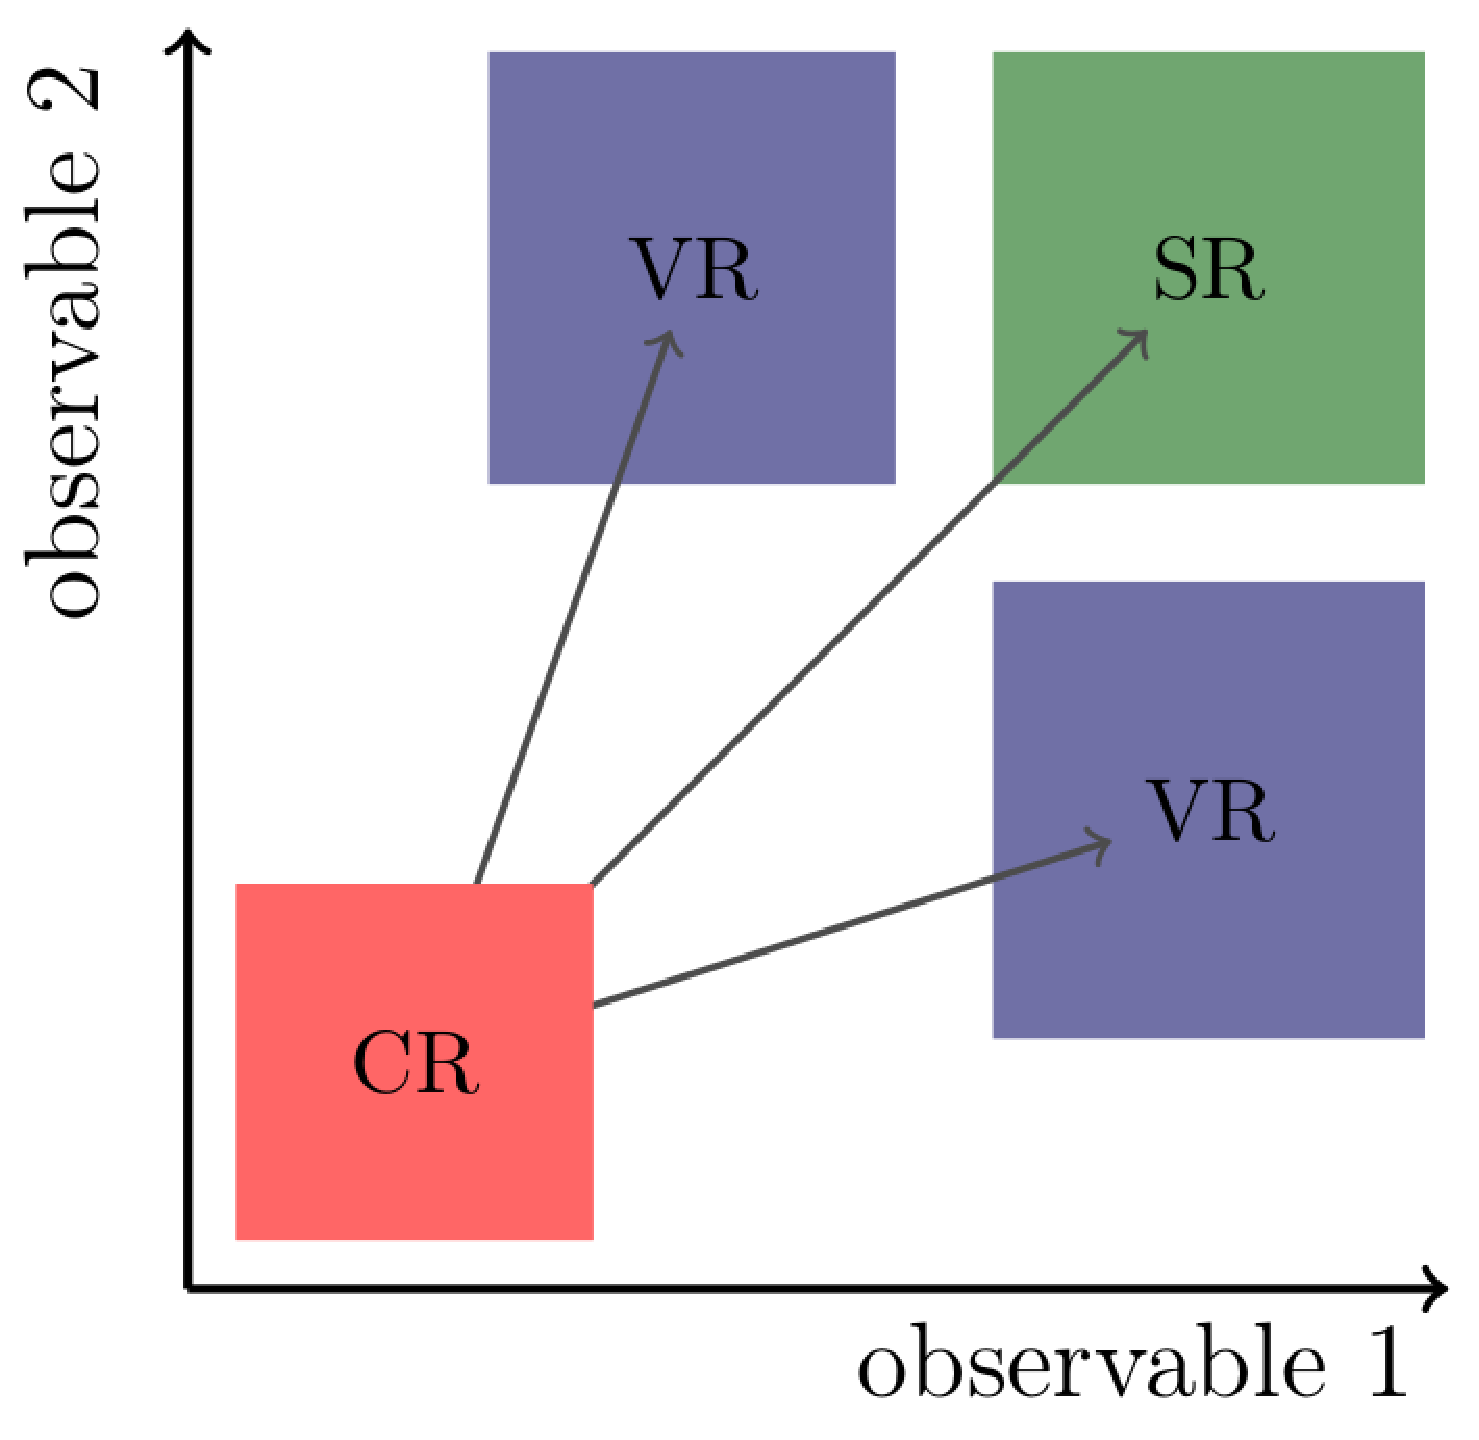
\includegraphics[width=0.40\textwidth]{regions.eps}
\caption{Esquema del diseño de las regiones de señal (SR), control (CR) y validación (VR) en términos de dos observables arbitrarios.}
% \vspace{0.2cm}\footnotesize\textbf \sl{...}\vspace{0.2cm}
\label{regions}
\end{figure}

\section{Selección de eventos}

DATOS DE LA TESIS DE FRAN?


